% !TEX root = ../main.tex

\subsection{ATLAS Humanoid Robot}

\ldots

\begin{figure}[t]
\centering
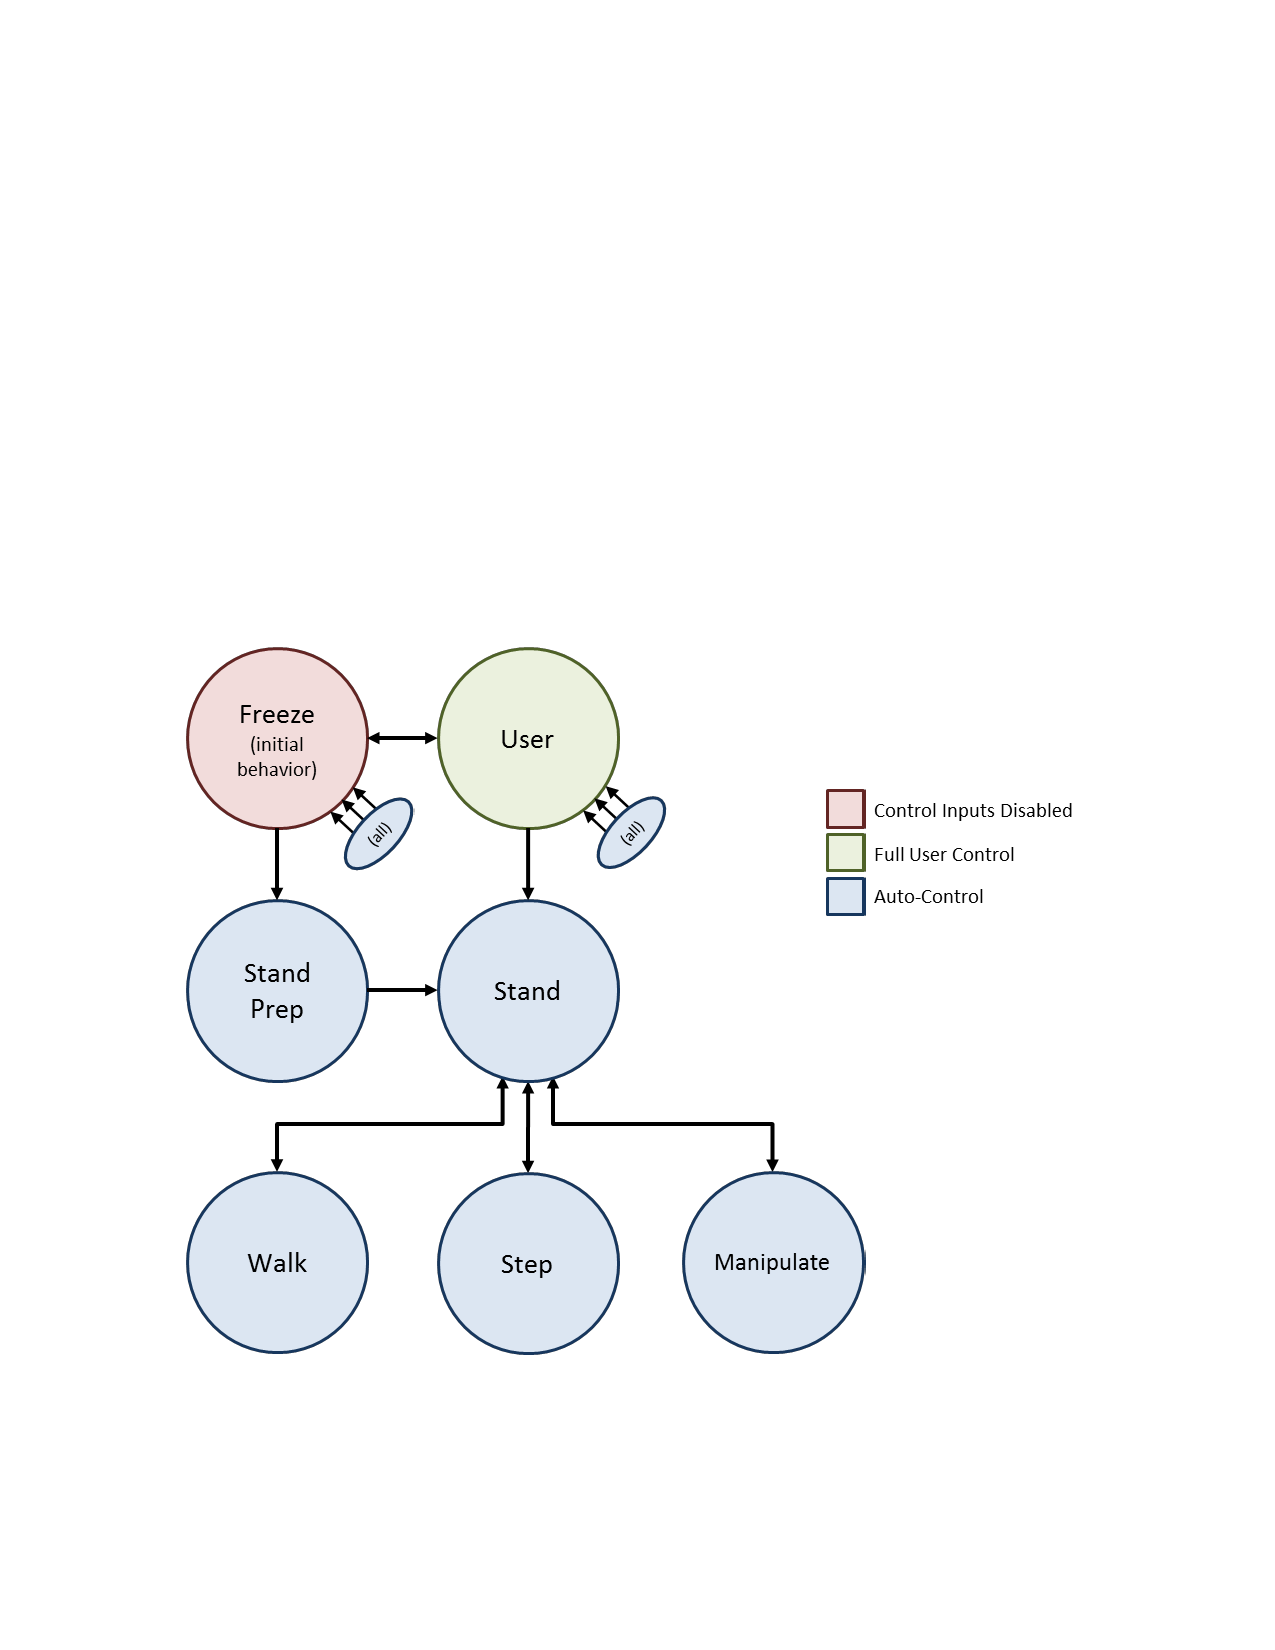
\includegraphics[width=0.95\columnwidth,clip]{./img/control_modes_ts.pdf}
\caption{
	\todo[inline, caption = {Create a simple control mode TS figure}]{Placeholder! Create two subfigures depicting a simple control mode TS and ATLAS doing something.}
}
\label{Fig:ControlModeTS}
%\vspace{-3 pt}
\end{figure}

\subsection{Team ViGIR's Approach to High-level Control}

\ldots

\subsection{Linear Temporal Logic and Reactive LTL Synthesis}

\ldots